\documentclass[12pt]{article}
\usepackage{amsmath}
\usepackage{graphicx}
\usepackage{hyperref}

\begin{document}

\title{Hub Identification in Global Air Network}
\author{
}
\date{}
\maketitle

\begin{table}[h!]
	\centering
	\begin{tabular}{|c|c|}
		\hline
		\textbf{Lab}                  & \textbf{Open Ended 14} \\
		\hline
		\textbf{Muhammad Hamza}       & 407251                 \\
		\hline
		\textbf{Aqsa Batool}          & 413777                 \\
		\hline
		\textbf{Ahmed Mohiuddin Shah} & 415216                 \\
		\hline
		\textbf{Section}              & BSCS-12-A              \\
		\hline
	\end{tabular}
\end{table}

\newpage

\section*{Introduction}
This report provides a detailed summary of the methodologies, key extractions, and results obtained during the analysis of the global air network. The primary objective was to identify critical hubs using centrality measures and predictive models. Two centrality measures, \textbf{Closeness Centrality} and \textbf{Betweenness Centrality}, were employed due to their promising results during preprocessing.

\begin{figure}[h!]
	\centering
	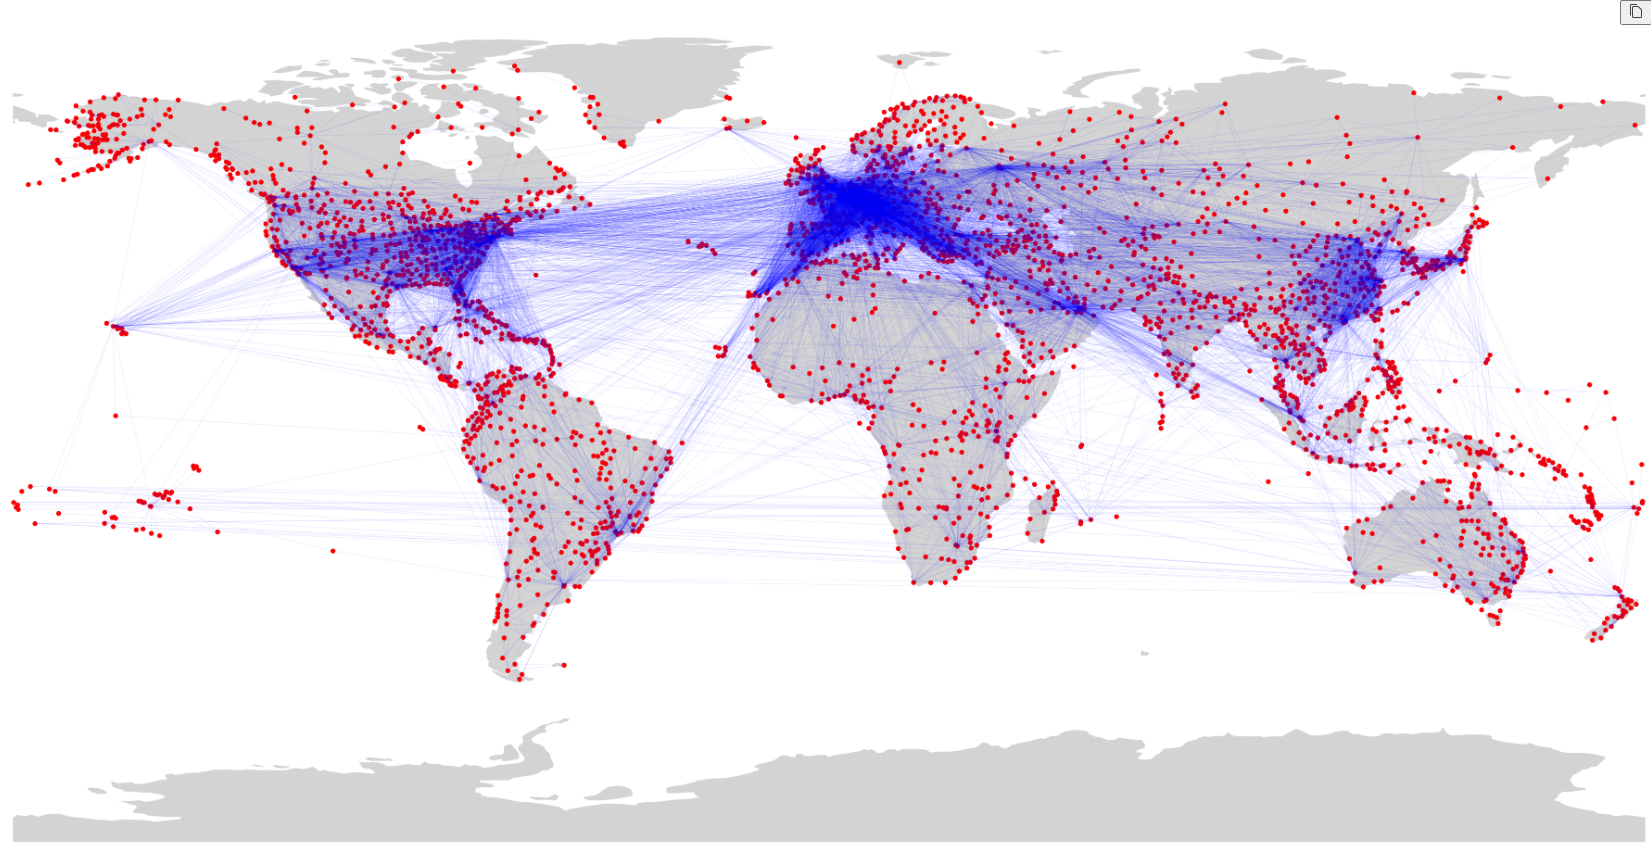
\includegraphics[width=1\textwidth]{figures/complete.png}
	\caption{Global Air Network}
	\label{fig:air_network}
\end{figure}

\section*{Centrality Measures Used}
\subsection*{Closeness Centrality}
Closeness Centrality quantifies how quickly information can spread from a node to all other nodes in the network. It is particularly useful for:
\begin{itemize}
	\item Identifying nodes that have the shortest average path to other nodes.
	\item Highlighting nodes that can act as efficient communicators within the network.
\end{itemize}

\subsection*{Betweenness Centrality}
Betweenness Centrality measures the number of shortest paths passing through a node. It is essential for:
\begin{itemize}
	\item Identifying nodes that act as bridges or critical intermediaries.
	\item Highlighting nodes with significant control over information flow.
\end{itemize}

\subsection*{Degree Centrality}
Degree Centrality was also calculated to provide a baseline comparison with the other centrality measures. However, it was not used in the predictive models due to its limited ability to capture the importance of nodes in the network.

\subsection*{Eigenvector Centrality}
Eigenvector Centrality was considered as an alternative centrality measure. However, it did not offer much improvement over the other measures and was not included in the final analysis although it was faster to run.

The betweenness and Closeness measures were selected because their preprocessing results indicated strong correlations with critical hubs in the network.

\section*{Data Preprocessing}
The data preprocessing steps included:
\begin{itemize}
	\item \textbf{Data Collection:} Airline routes data was obtained from the OpenFlights dataset.
	\item \textbf{Data Cleaning:} Invalid or missing entries were removed, and the dataset was filtered to include only relevant information.
	\item \textbf{Graph Construction:} The air network was represented as a graph, with airports as nodes and flight routes as edges.
	\item \textbf{Centrality Calculation:} Closeness, Betweenness, and Degree centrality were calculated for each node in the network.
	\item \textbf{Feature Extraction:} Centrality measures were used as features for training predictive models. We also created Features such as major airlines for each airport, incoming and outgoing flights, and the number of routes and also the lengths of routes.
\end{itemize}

\section*{Model Results}
The following metrics were used to evaluate the performance of predictive models for identifying hubs based on centrality measures:
\begin{itemize}
	\item Mean Squared Error (MSE)
	\item Accuracy
	\item R\textsuperscript{2} Score
	\item Cross-Validation Scores
\end{itemize}

\subsection*{Closeness Centrality}
\begin{verbatim}
Mean Squared Error: 0.00034099487277159394
Accuracy: 0.8490904453097192
R \textsuperscript{2} Score: 0.8490904453097192
Cross-Validation Scores: [0.74864875, 0.84155135, 0.7859669, 0.74380287, 0.66345503]
Mean Cross-Validation Score: 0.7566849804042652
\end{verbatim}
\textbf{Implications:} The high accuracy and R\textsuperscript{2} score indicate that closeness centrality is a reliable predictor for identifying key hubs that efficiently connect the network.

\subsection*{Betweenness Centrality}
\begin{verbatim}
Mean Squared Error: 9.487119502115798e-06
Accuracy: 0.6965426040693008
R\textsuperscript{2} Score: 0.6965426040693008
Cross-Validation Scores: [0.70046918, 0.63002486, 0.60691534, 0.69054177, 0.25956295]
Mean Cross-Validation Score: 0.5775028193707866
\end{verbatim}
\textbf{Implications:} While the accuracy is lower than closeness centrality, betweenness centrality provides insights into nodes that act as crucial intermediaries, making it valuable for identifying bottlenecks or bridges.

\section{Visualization of Predictions VS Actual Data}
\subsection*{Closeness Predictions}
\begin{figure}[h!]
	\centering
	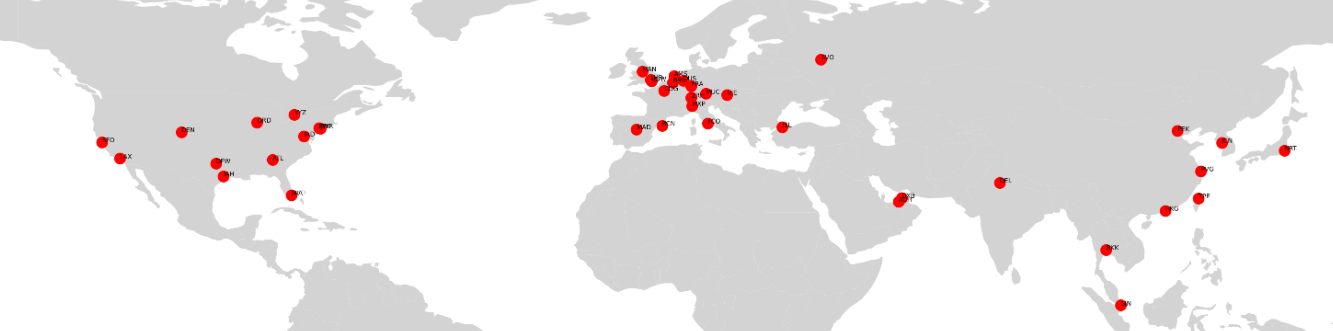
\includegraphics[width=1\textwidth]{figures/c_pred.png}
	\caption{Predictions vs. Actual Data}
	\label{fig:closeness_predictions}
\end{figure}

\subsection*{Closeness Real Values}
\begin{figure}[h!]
	\centering
	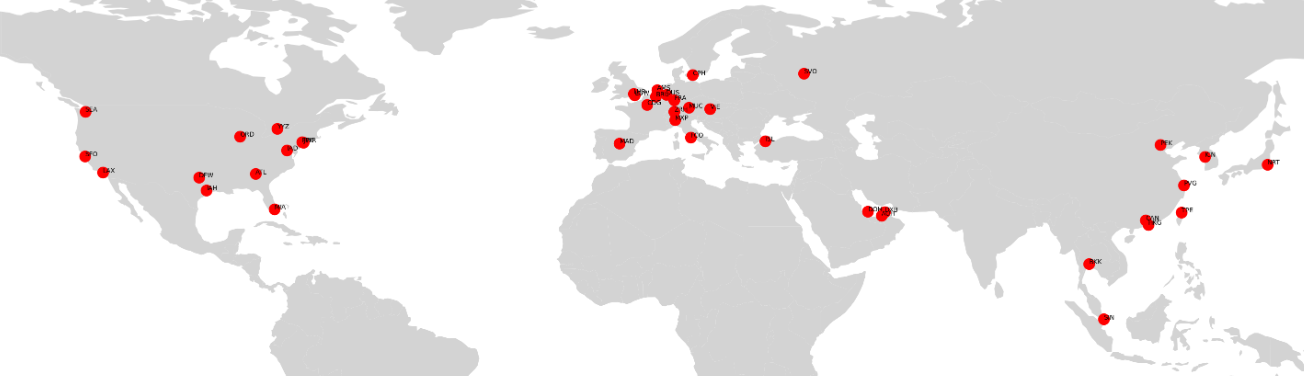
\includegraphics[width=1\textwidth]{figures/c.png}
	\caption{Predictions vs. Actual Data}
	\label{fig:closeness}
\end{figure}

\newpage
\subsection*{Betweenness Predictions}
\begin{figure}[h!]
	\centering
	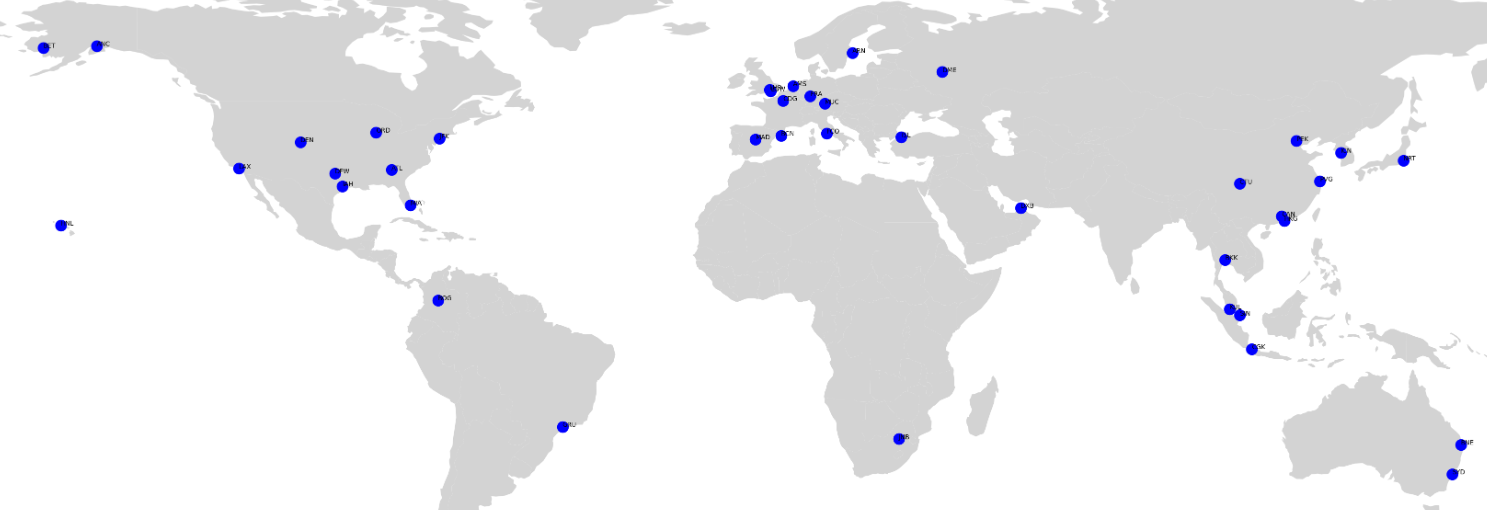
\includegraphics[width=1\textwidth]{figures/b_pred.png}
	\caption{Predictions vs. Actual Data}
	\label{fig:betweennesspredictions}
\end{figure}

\subsection*{Betweenness Real Values}
\begin{figure}[h!]
	\centering
	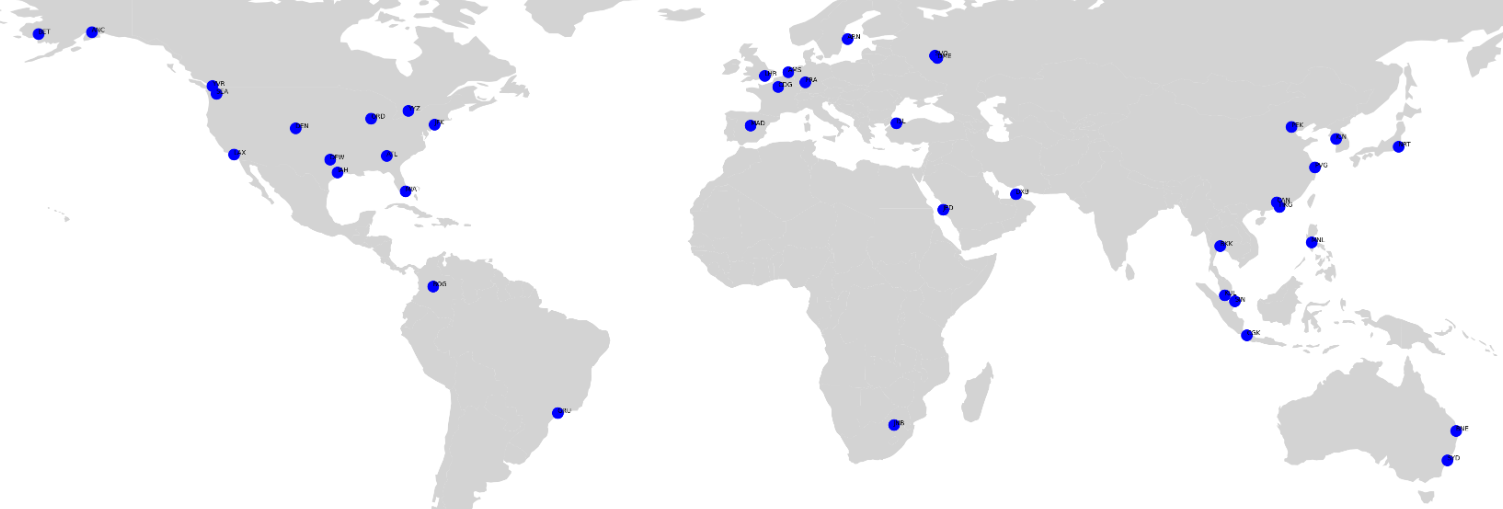
\includegraphics[width=1\textwidth]{figures/b.png}
	\caption{Predictions vs. Actual Data}
	\label{fig:betweenness}
\end{figure}

\newpage

\section*{Key Techniques Used}
\begin{itemize}
	\item \textbf{Graph Representation:} The air network was represented as a graph, with airports as nodes and flight routes as edges.
	\item \textbf{Centrality Analysis:} Closeness and Betweenness centrality were calculated for each node to determine their importance in the network.
	\item \textbf{Machine Learning Models:} Predictive models were trained using features derived from centrality measures to identify critical hubs.
	\item \textbf{Cross-Validation:} Ensured robust evaluation of model performance.
\end{itemize}

\section*{Challenges and Solutions}
\begin{itemize}
	\item \textbf{Graph Size and Complexity:} Analyzing a large, global network posed computational challenges. Efficient graph libraries, such as \texttt{NetworkX}, and parallel computation were used to overcome this.
	\item \textbf{Feature Selection:} Selecting meaningful features was critical for accurate predictions. Centrality measures were chosen based on their theoretical relevance and preprocessing results.
\end{itemize}

\section*{Conclusions and Recommendations}
The analysis demonstrated that:
\begin{itemize}
	\item Closeness Centrality is a reliable measure for identifying efficiently connected hubs.
	\item Betweenness Centrality is valuable for detecting critical intermediaries.
\end{itemize}
Airlines and airport authorities can leverage these insights to:
\begin{itemize}
	\item Optimize route planning and resource allocation.
	\item Identify critical airports for infrastructure investment.
\end{itemize}

Future work could include incorporating additional data, such as flight delays, passenger volumes, and economic indicators, to enhance the analysis and provide more actionable insights.

\end{document}
